\section{Discussion}
\note{
    \begin{itemize}
        \item Notes...
    \end{itemize}
}

\metroset{block=transparent}

\subsection{Unmitigated Threats}

\begin{frame}{Exploring Unmitigated Threats}
    \begin{columns}[T,onlytextwidth]
        \column{0.47\textwidth}
        \pause

        \begin{block}{Cryptography Exploit}
            \begin{itemize}

                \item Beacon not dependent on any algorithm
            \end{itemize}
        \end{block}
        \pause
        \begin{block}{Eclipse Attacks}
            \begin{itemize}
                \item Have multiple connections to outside world
            \end{itemize}
        \end{block}

        \column{0.47\textwidth}
        \pause
        \begin{block}{Operator Shutdown}
            \begin{itemize}
                \item Only disrupts use cases
            \end{itemize}
        \end{block}

        \pause
        \begin{block}{Input Flooding}
          \begin{itemize}
              \item Rate limiting
              \item Proof-of-Work puzzle
          \end{itemize}
        \end{block}

    \end{columns}
\end{frame}
\note{
    Notes...
}

\subsection{Alternative Delay Functions}

\begin{frame}{Alternative Delay Functions}
    \centering
    A dedicated ASIC to compute \emph{sloth} may be faster.
    \\
    \vspace{1cm}
    Adversary with ASIC must also be able to execute an attack.
\end{frame}
\note{
    \begin{itemize}
        \item aaaa
    \end{itemize}
}

\begin{frame}{Alternative Delay Functions}
    \centering
    \textbf{Two solutions:}

    \vspace{.5cm}
    
    \begin{columns}[T, onlytextwidth]
        \column{0.47\textwidth}
        \begin{block}{Use Memory-Hard Delay Function}
            \begin{itemize}
                \item ASICs have limited memory.
                \item Requiring memory in delay function makes ASICs infeasible
            \end{itemize}
        \end{block}

        \column{0.47\textwidth}
        \begin{block}{Change Delay Function}
            \begin{itemize}
                \item ASIC: expensive and hard-wired
                \item Beacon: Changing/permutating delay function is free
            \end{itemize}
        \end{block}
    \end{columns}
\end{frame}
\note{
    \begin{itemize}
        \item aaaaa
    \end{itemize}
}



\begin{frame}{Rational Trust}

    \centering
    \enquote{The beacon is secure if there are (at least)\\\textbf{two non-colluding disjoint sets of input}}
    
    \pause
    \vspace{.3cm}
    \begin{tikzpicture}
        \draw[ultra thick] (0,0) ellipse (1 and 2)
            (4,0) ellipse (1 and 2);
        % \clip (0,0) ellipse (1 and 2) (4,0) ellipse (1 and 2);
        \only<2>{
            \fill (0.5, 0.9) circle(1.5pt);
            \fill (-0.3, 1.3) circle(1.5pt);
            \fill (-0.2, -1.4) circle(1.5pt);
            \fill (-0.7, 0.1) circle(1.5pt);
        }
        \only<1-4>{
            \fill (0.3, -0.4) circle(1.5pt);
        }
        \only<4>{
            \coordinate (end) at (0.3, -0.4);
            \coordinate (start) at (1.5, -1);
            \draw[-latex, shorten <=3pt, thick, draw=red] (start) -- (end);
        }

        \fill (3.7, 1.4) circle(1.5pt);
        \fill (4.2, -1.6) circle(1.5pt);
        \fill (3.7, -0.5) circle(1.5pt);
        \fill (4.7, 0.1) circle(1.5pt);
    \end{tikzpicture}

\end{frame}
\note{
    Notes...
}

\subsection{Practicalities}

\begin{frame}{Practicalities: Stopping in a Fair Way}
    \textbf{Desirable beacon properties:}
    \begin{itemize}
        \item High output frequency
        \item Long input collection time
    \end{itemize}

    \vspace{.7cm}
    \centering
    \pause
    Solution: Ceremonies on top of beacon

    \vspace{.3em}
    \pause
    Standardize this common pattern

\end{frame}
\note{
    Notes...
}

\begin{frame}{Practicalities: Extending Trust into the Reality}
    How can we ensure that the lottery pays the money?
    \pause
    \begin{itemize}
        \item Trust them
        \pause
        \item Cryptocurrencies and smart contracts
    \end{itemize}
\end{frame}
\note{
    Notes...
}

\begin{frame}{Summary}
    Succinct beacon design and implementation
    \begin{itemize}
        \item Enumerate threats
        \item Describe usage of beacon in context
        \item Of more technical nature:
        \begin{itemize}
            \item Parallelized pipeline
            \item Early release of inputs (CCO)
            \item Multiple input/output channels
            \item Usage of Merkle trees
        \end{itemize}
    \end{itemize}
\end{frame}
\note{
    Notes...
}
